\chapter{Hardware}
\label{Hardware}
\section{Überblick}

Vielleicht könnte dieses Schema hier viel gewinnbringender eingefügt werden als im Abschnitt Grobkonzept?

\begin{figure}[H]
	\centering
	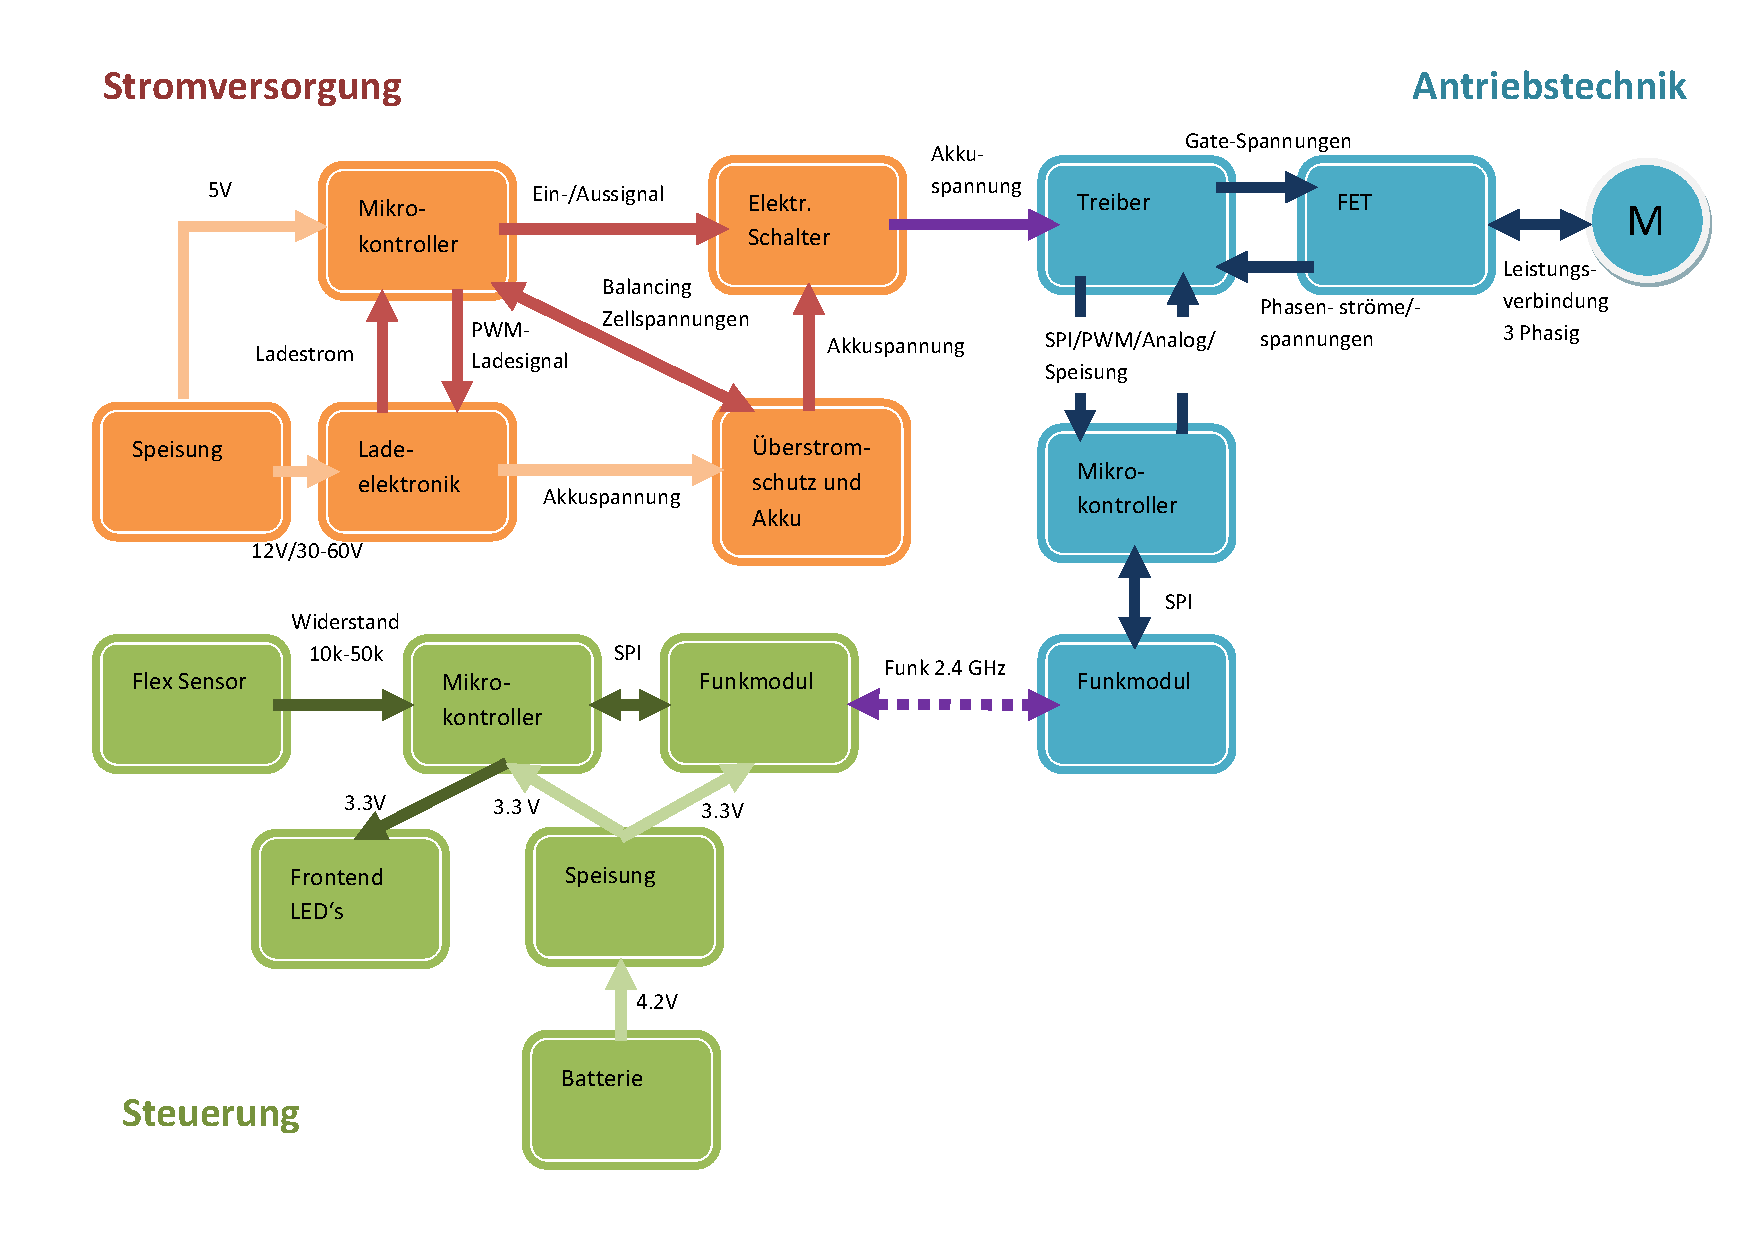
\includegraphics[width=1\linewidth]{images/Grobkonzept_Blockschaltbild_detailliert}
	\caption[Detailliertes Blockschaltbild]{Detailliertes Blockschaltbild}
	\label{fig:grobkonzeptblockschaltbilddetailliert_2}
\end{figure}


\section{Steuerung - Magic-Glove}
\label{HW_MagicGlove}

\section{Stromversorgung}
\label{HW_Stromversorgung}
An die Stromversorgung werden einige Anforderungen gestellt. So muss sie für die Motorsteuerung grosse Ströme mit bis zu 50A liefern können. Dabei muss die Spannung der Zellen kontinuierlich überprüft werden um ein Tiefentladen zu verhindern. Des Weiteren wird eine Standby-Killer Schaltung implementiert und dessen Funktion erklärt.\\
Um das Board einfach laden zu können ohne jedes Mal den Akku ausbauen zu müssen, hat sich unser Team entschieden eine Akku Ladeschaltung einzubauen. Diese muss die Zellen balancen und sie vor Überspannung bzw. Überladung schützen. 
\todo{Leserführung was kommt nun}
\subsection*{Balancing}
- ...
\subsection*{Ladeelektronik}
-	PWM zu Strom Schaltung\\
-	Selbsthaltung\\
-	Linearregler

\subsection*{Mikrocontroller}
An den Mikrocontroller werden verschiedene Anforderungen gesetzt.
In folgender Tabelle \ref{tabGPIObat} werden die General Purpose Input Output (GPIO) Anforderungen an den Mikrocontroller aufgelistet.
\begin{center}
	\begin{tabular}{|c|c|c|c|}
		\hline 
		Beschreibung & Anforderung & Input/Output & Anzahl \\ 
		\hline 
		Überwachung der Zellen & Analog & Input & 6 \\ 
		\hline 
		Überwachen des Ladestroms &	Analog & Input & 1 \\ 
		\hline 
		Überwachen der Eingangsspannung & Analog & Input & 1 \\ 
		\hline 
		&  &  &  \\ 
		\hline 
		Entladen der Zellen (Balanceing) & Digital  & Output & 6 \\ 
		\hline 
		Anzeige des Ladezustands (LED) & Digital & Output & 3 \\ 
		\hline 
		Schalten des Ausgang Stroms zum Motor & Digital & Output & 1 \\ 
		\hline 
		Selbsthaltung des Mikrocontrollers & Digital & Output & 1 \\ 
		\hline 
		&  &  &  \\ 
		\hline 
		Regelung des Ladestroms & PWM & Output & 1 \\ 
		\hline 
		Kommunikation SPI Schnittstelle MISO/MOSI/SCK & Serial & In/Output & 3 \\ 
		\hline 
	\end{tabular} 
	\captionof{table}{GPIO Anforderungen für den Mikrocontroller}
	\label{tabGPIObat}
\end{center}
Für die Regelung der Stromversorgung wird der Mikrocontroller ATmega328P-AU verwendet.
\subsection*{Zellmessung}
Die Messung der Zellen durchlief während der Entwicklungsphase mehrere Änderungen. Die Zellen sind in Serie geschaltet, um dem Motor genügend Spannung zur Verfügung zu stellen. Mit einer Zellenspannung von 4.15V pro Zelle liegt am obersten Punkt (Anode der Zelle 6) eine Spannung von 24,9V. Da die Spannung an den Eingängen des Mikrocontrollers nicht seine Speisespannung übersteigen sollte, mussten diese Spannungen verringert werden. In unserem Fall beträgt die maximale Spannung am Eingang 5V. Die erste Idee war, wie in Abb.\ref{fig:zellmessung} links oben zu sehen, mit einfachen Spannungsteiler die Spannungen so zu skalieren, dass die Maximalspannung nicht überschritten wird. 
\begin{figure} [H]
	\centering
	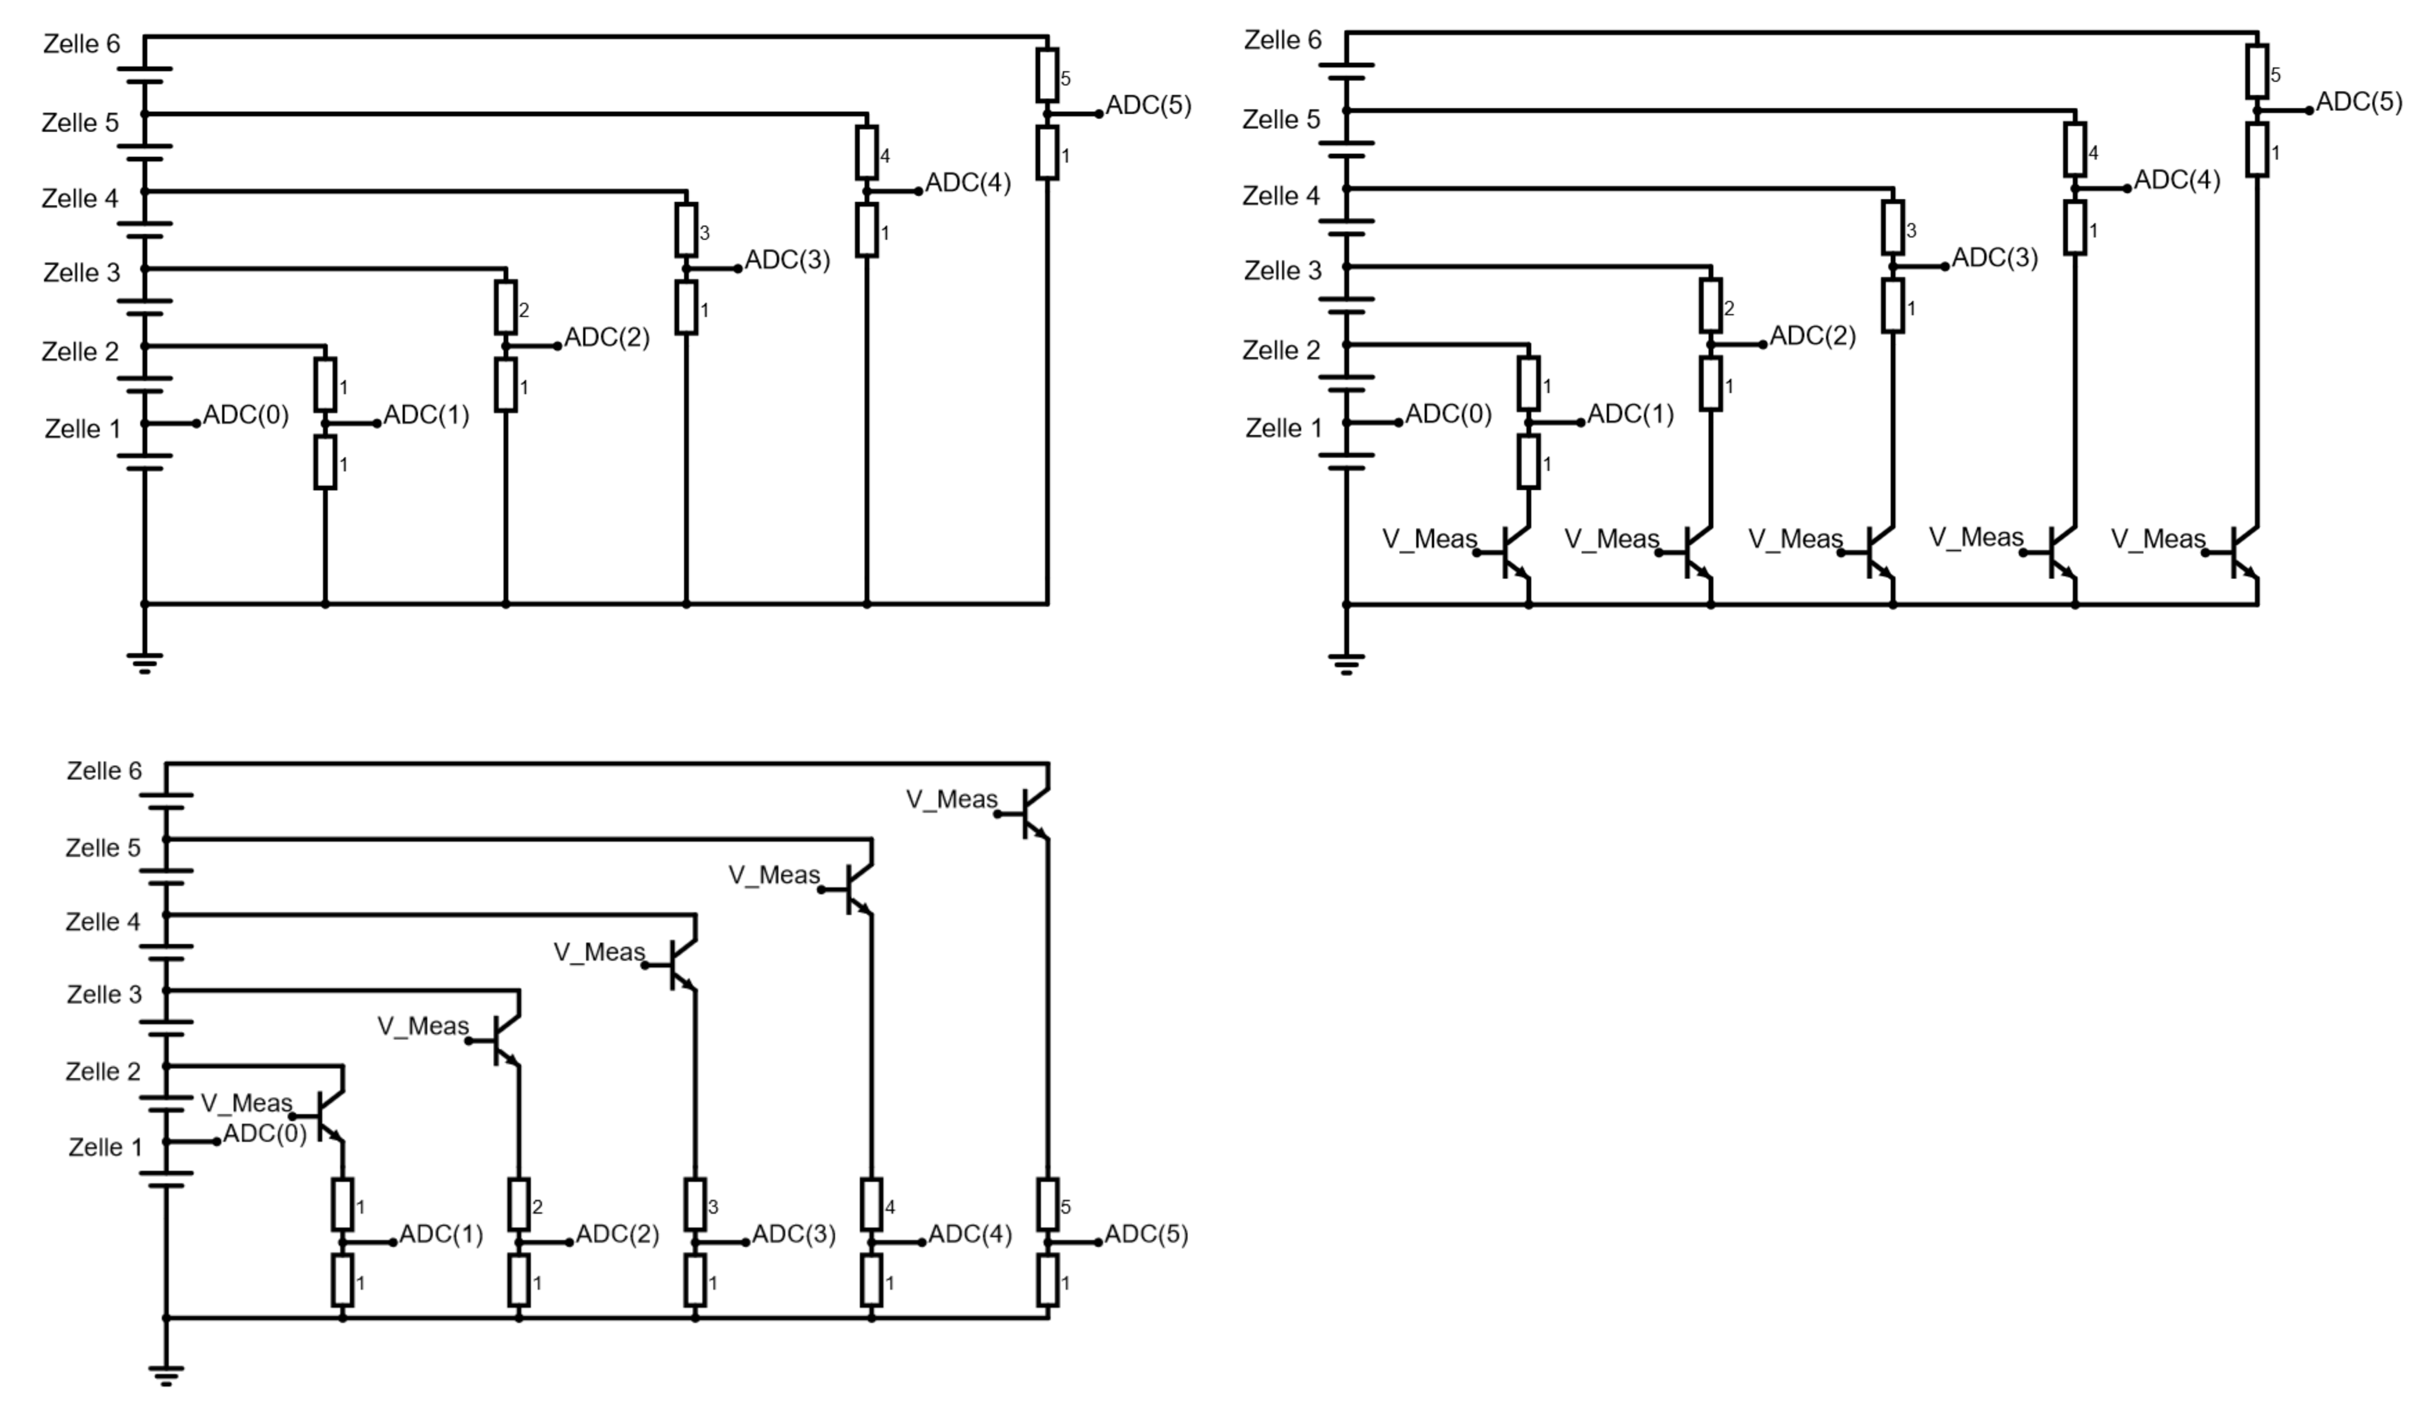
\includegraphics[width=1\linewidth]{images/Zellmessung}
	\caption{Messung der Zellen - verschiedene Arten}
	\label{fig:zellmessung}
\end{figure}
\todo{besserer Titel für Abb.}
Der Nachteil dieser Schaltung ist, dass die Zellen durch die Spannungsteiler kontinuierlich entladen werden. Somit können bei einem längeren Nichtgebrauch die Akkuzellen entladen oder sogar tiefentladen sein. \\
Um dies zu verhindern wurde der zweite Entwurf auf der rechten Seite der Abb.\ref{fig:zellmessung} entwickelt. Dieser unterbricht mit den Transistoren den Entladestromkreis über den Widerständen. Die Transistoren werden übersteuert, um sie als Schalter zu verwenden und den durch die UCE \todo{hä? bzw. Formatierung notwendig? U$_{CE}$ --> U\_collector\_emitter aaahhhaaa} Spannung entstehende Fehler zu verkleinern. Dieser tritt je nach Sättigungsspannung der Transistoren jedoch immer noch auf und ist durch die unterschiedlichen Bauarten nur schwer zu korrigieren. Der zweite grosse Nachteil und gleichzeitig Killerkriterium für diese Schaltung war, dass durch das Unterbrechen des Spannungsteiler Stromkreises an den ADC Ausgängen wieder die Zellenspannung anliegt. Dadurch würden sich die Zellen über die Ableitdiode am Eingang des Mikrocontrollers entladen und diese \todo{diese = die Ableitdiode?} voraussichtlich zerstören. \\
Dies könnte verhindert werden, indem der Stromkreis oberhalb der ADC Eingängen unterbrochen wird. Dies ist in der linken unteren Schaltung der Abb.\ref{fig:zellmessung} gezeichnet. Dadurch wären die Eingänge vor Überspannung geschützt. Aber auch diese Schaltung bringt diverse Nachteile. So fliesst beim geschlossenen Zustand der Basis-Emitter Strom durch den Spannungsteiler. Dies verfälscht die Messresultate. Zusätzlich muss zwischen Basis und Emitter eine Schaltspannung von mindestens 0.7V sein. Dazu müsste die Schaltspannung 0.7V über der Zellspannung liegen, was nur mit grossem Aufwand erreichbar wäre. 
In einem Teamentscheid wurde die erste Methode gewählt, da sie die genausten Messungen liefert und die Entladung der Zellen bei einer durchschnittlichen Benutzung des Boards nie \todo{ev.:nicht ?} zu tragen kommt.

\section{Motoransteuerung}
\label{HW_Motoransteuerung}
\subsection*{Treiber IC und Speisung}
\subsection*{Endstufe (H-Brücke)}
\subsection*{Messschaltung}
\subsection*{Mikrocontroller}

